\chapter{Gaussian Mixture Models}
\label{ch:gmm}

\chapterref{speaker-recognition-systems} briefly discussed the use of models $\lambda_i$ to perform an identification process and models $\lambda_{hyp}$ and $\lambda_{bkg}$ for a claimed speaker and for a background composed of all enrolled speakers, respectively, to a verification process. As the features from the speech signal (see \chapterref{feature-extraction}) have unknown values until the moment of extraction, it is reasonable to model the ASR system to accept random values.

For all sorts of probability distributions, the gaussian (or normal) is the one that best describes the behavior of a random variable of unknown distribution, as demonstrated by the central limit theorem. Its equation for a D-dimensional space is

\begin{equation}
    \pdf{\dvec{x}} = p(\dvec{x},\dvec{\mu},\dvec{\Sigma}) = \dgaussian{x}{\mu}{\Sigma},
    \label{eq:gaussian}
\end{equation}

\noindent where $\dvec{x}$ is a $D$-dimensional input vector, $\dvec{\mu}$ the $D$-dimensional vector of means, $\dvec{\Sigma}$ the $D \times D$ matrix of covariances, $\dvec{|\Sigma|}$ the determinant of $\dvec{\Sigma}$, and $(\dvec{x} - \dvec{\mu})'$ the transposed of the colum-matrix $(\dvec{x} - \dvec{\mu})$.

\section{Definition}
\label{sec:gmm-definition}

A weighted sum of $\pdf{\dvec{x}}$'s is used to model the ASR system, estimating the composition that best represents the training data. This weighted sum is named Gaussian Mixture Model (GMM), first used for speaker recognition in \refbib{Reynolds}{reynolds.1992}, and is given by

\begin{equation}
    \postpdf{\dvec{x}}{\lambda} = \sum_{i=1}^M w_i\pdfi{\dvec{x}},
    \label{eq:gaussian_mixture}
\end{equation}

\noindent where $M$ is the size of the distribution used, $\sum_{i=1}^M w_i = 1$, and $\lambda = \{w_i, \dvec{\mu}_i, \dvec{\Sigma}_i\}$ is the model representation, for $i = 1, ..., M$. Each Gaussian in each model has its own covariance matrix (nodal covariance). Applying \equationref{gaussian} to \equationref{gaussian_mixture}, the likelihood for the GMM is

\begin{equation}
    \postpdf{\dvec{x}}{\lambda} = \dgaussianmixture.
    \label{eq:likelihood_gmm}
\end{equation}

The idea behind the use of a GMM as a model for a speaker $\mathcal{S}$ is to achieve a $\lambda$ that maximizes the likelihood when applied to features $\dvec{X}$ extracted from a speech signal produced by $\mathcal{S}$. This value is found by a Maximum Likelihood Estimation (MLE) algorithm. For a sequence of T training vectors $\dvec{X} = \{\dvec{x}_t\}$, the GMM likelihood can be written as

\begin{equation}
    \postpdf{\dvec{x}}{\lambda} = \prod_{t=1}^T \postprob{\dvec{x}_t}{\lambda}.
    \label{eq:likelihood_gmm_mle}
\end{equation}

\noindent Unfortunately, this expression is a nonlinear function of the parameters $\lambda$ and direct maximization is not possible, \refbib{Reynolds}{reynolds.1995c}, leading to estimate $\postpdf{\dvec{x}}{\lambda}$ iteratively using the Expectation-Maximization (EM) algorithm.

In this paper, the GMM that models a single speaker will be reffered to as Single Speaker Gaussian Mixture Model (SSGMM), as initially cited in \sectionref{gmm}.

\section{Expectation-Maximization}
\label{sec:em}

The idea of the EM algorithm is to estimate a new model $\lambda^{(j+1)}$ from a previous model $\lambda^{(j)}$, that obeys $\postpdf{\dvec{x}}{\lambda^{(j+1)}} \geq \postpdf{\dvec{x}}{\lambda^{(j)}}$, approximating the GMM to the training data at each iteration until some convergence threshold is reached. The algorithm is composed of 2 steps, an expectation of the \emph{a posteriori} probabilities for each distribution $i$, and a maximization step, when the parameters $w_i$, $\dvec{\mu}_i$ and $\dvec{\Sigma}_i$ are updated. The following description of the steps uses a $\lambda$ with \textbf{diagonal}\footnote{As stated in \refbib{Reynolds et. al.}{reynolds.quatieri.dunn.2000}, diagonal covariance matrix GMMs outperform and are more computationally efficient than full covariance matrix GMMs. Also, the density modeling of an $M$-th order full covariance matrix GMM can equally well be achieved using a larger order diagonal covariance.} $\dvec{\Sigma}_i$ (i.e., change the $D \times D$ matrix $\dvec{\Sigma}_i$ for a $D$-dimensional vector $\dvec{\sigma}_i^2$ of variances).

\begin{figure}[ht]
    \centering
    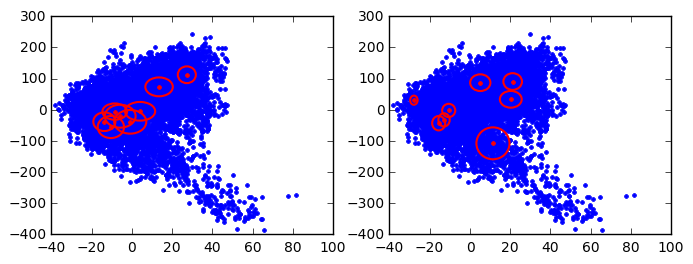
\includegraphics[width=\textwidth]{chapters/gmm/em_algorithm}
    \caption{Features before (left), partitioned using k-means, and after (right) the EM algorithm. Only the first deviation is shown.}
    \label{fig:em_algorithm}
\end{figure}

\subsubsection*{E-Step}

The \textbf{expectation step} consists of estimating the \emph{a posteriori} probabilities $\postprob{i}{\dvec{x}_t, \lambda}$ for each distribution $i$ and each feature vector $\dvec{x}_t$, defined as

\begin{equation}
    \postprob{i}{\dvec{x}_t, \lambda} = \postprob{i}{\dvec{x}_t} = \frac{w_i p_i(\dvec{x}_t)}{\sum_{k=1}^M w_k p_k(\dvec{x}_t)}.
    \label{eq:e-step-posterior}
\end{equation}

\subsubsection*{M-Step}

In the \textbf{maximization step} the model is updated by recalculation of the parameters $w_i, \dvec{\mu}_i$ and $\dvec{\Sigma}_i$, and the algorithm guarantees that each new $\lambda^{(j+1)}$ represents the training data better than the previous ones. From \refbib{Reynolds}{reynolds.1995c}, the updates of $w_i$, $\dvec{\mu}_i$ and $\dvec{\sigma}_i^2$ are given by the equations below.

\noindent\\\textbf{Weights:}

\begin{equation}
    \overline{w}_i = \frac{1}{T} \sum_{t=1}^T \postprob{i}{\dvec{x}_t, \lambda},
    \label{eq:m-step-weight}
\end{equation}

\noindent\\\textbf{Means:}

\begin{equation}
    \overline{\dvec{\mu}}_i = \frac{\sum_{t=1}^T \postprob{i}{\dvec{x}_t, \lambda} \dvec{x}_t}{\sum_{t=1}^T \postprob{i}{\dvec{x}_t, \lambda}},
    \label{eq:m-step-means}
\end{equation}

\noindent\textbf{Variances:}

\begin{equation}
    \overline{\dvec{\sigma}}_i^2 = \frac{\sum_{t=1}^T \postprob{i}{\dvec{x}_t, \lambda} \dvec{x}_t^2}{\sum_{t=1}^T \postprob{i}{\dvec{x}_t, \lambda}} - \overline{\dvec{\mu}}_i^2.
    \label{eq:m-step-variances}
\end{equation}
\\

This algorithm trains the GMMs used in the ASR system shown in sections \sectionrefcomp{speaker-identification} and \sectionrefcomp{speaker-verification} and previously described in \sectionref{gmm-definition}. \figureref{em_algorithm} shows the mixture before and after the training.

\section{Universal Background Model}
\label{sec:ubm}

An Universal Background Model-Gaussian Mixture Model (UBM-GMM), shortened to UBM, is a GMM composed of features from all enrolled speakers. The idea is to generate a model $\lambda_{bkg}$ where common characteristics present in the corpus are well represented. Then, a speech mostly composed of common characteristics from enrolled speakers is more difficult to pass the likelihood ratio test (see \equationref{likelihood-ratio-test}).

There are many configurations for an UBM, but, as it is possible to see in \refbib{Reynolds et. al.}{reynolds.quatieri.dunn.2000}, male and female speakers present distinct vocal traits and are better represented when trained separately. Also, female voices have more intrasimilarities than males, leading to more distinct male configurations. The $M$-th order UBM in this study is created merging trained male and female models, both of order $M/2$ (see \figureref{ubm-diagram}).

\begin{figure}[ht]
    \centering
    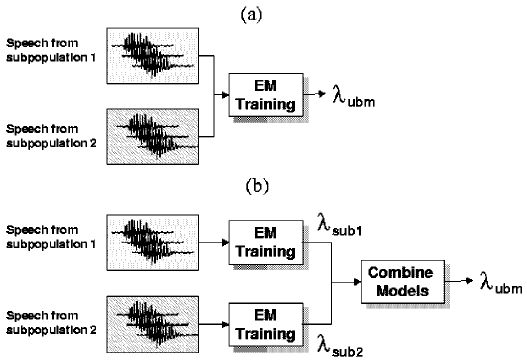
\includegraphics[width=0.55\textwidth]{chapters/gmm/ubm-diagram}
    \caption{UBM with gender trained (a) together and (b) separately and combined, \refbib{Reynolds et. al.}{reynolds.quatieri.dunn.2000}.}
    \label{fig:ubm-diagram}
\end{figure}

As shown in \sectionref{speaker-verification}, the likelihood ratio test is performed using the models $\lambda_{hyp}$ and $\lambda_{bkg}$. The default ASR system is a SSGMM-UBM system, turning \equationref{score_of_X} in

\begin{equation}
    \Lambda(\dvec{X}) = \log p(\dvec{X}|\lambda_{SSGMM}) - \log p(\dvec{X}|\lambda_{UBM}).
    \label{eq:score_of_X_ssgmm_ubm}
\end{equation}

\section{Adapted Gaussian Mixture Model}
\label{sec:adapted-gmm}

As seen in \chapterref{speaker-recognition-systems} and in the previous sections, to perform the verification process a GMM for the claimed speaker and an UBM must be trained. Verify all speakers demands the training of SSGMMs for all enrolled speakers, a highly costly action (in time). An effective alternative is to take advantage of the well-trained $M$-th order UBM, since the SSGMMs and the UBM must have the same order to use \equationref{score_of_X_ssgmm_ubm}, and adapt its parameters to generate a new SSGMM for a speaker, \refbib{Brown et. al.}{brown.lee.spohrer.1983}. This technique provides a training faster than the SSGMM-UBM system (there is no loop such as in the EM algorithm) and tighter coupling between the speaker’s model and the UBM, \refbib{Reynolds et. al.}{reynolds.quatieri.dunn.2000}. The resultant GMM is named Single Speaker Adapted Gaussian Mixture Model (SSAGMM). Refactoring \equationref{score_of_X_ssgmm_ubm}, the log-likelihood ratio test for Adapted Gaussian Mixture Model (AGMM) is

\begin{equation}
    \Lambda(\dvec{X}) = \log p(\dvec{X}|\lambda_{SSAGMM}) - \log p(\dvec{X}|\lambda_{UBM}).
    \label{eq:score_of_X_ssagmm_ubm}
\end{equation}

The idea behind the Bayesian Adaptation\footnote{Also known as \textbf{maximum a posteriori} (MAP) estimation.} is to recalculate the gaussians from the UBM using only the desired speaker's features. If a gaussian represents the new data better than the old data, the change is relevant, as seen in \figureref{adapted_wmv}.

\begin{figure}[ht]
    \centering
    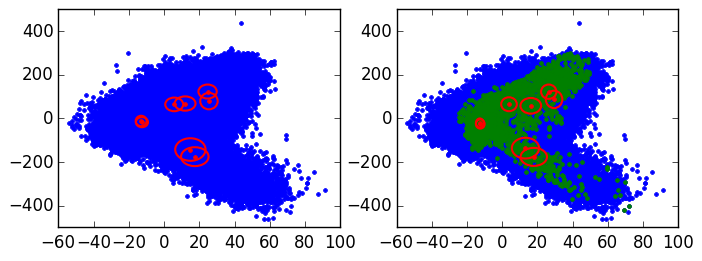
\includegraphics[width=\textwidth]{chapters/gmm/adapted_wmv}
    \caption{UBM trained (left) and weights, means and variances adapted for a female speaker (right). The blue dots are the background features and the green the speaker's.}
    \label{fig:adapted_wmv}
\end{figure}

The adaptation process is composed of two steps. The first is an expectation step, similar to the EM algorithm. Using $\postprob{i}{\dvec{x}_t}$ (see \equationref{e-step-posterior}) is possible to compute the sufficient statistics for the weight, mean, and variance parameters:\footnote{$\dvec{x}^2$ is shorthand for diag($\dvec{x}\dvec{x}'$).}

\begin{equation}
    n_i = \sum_{t=1}^{T} \postprob{i}{\dvec{x}_t}
    \label{eq:n_i}
\end{equation}

\begin{equation}
    E_i(\dvec{x}) = \frac{1}{n_i} \sum_{t=1}^{T} \postprob{i}{\dvec{x}_t} \dvec{x}_t
    \label{eq:E_x}
\end{equation}

\begin{equation}
    E_i(\dvec{x}^2) = \frac{1}{n_i} \sum_{t=1}^{T} \postprob{i}{\dvec{x}_t} \dvec{x}_t^2
    \label{eq:E_x2}
\end{equation}

Finally, these new sufficient statistics from the training data are used to update the old UBM sufficient statistics and adapt the parameters for mixture $i$ (see \figureref{adapted_wmv}) with the equations taken from \refbib{Reynolds et. al.}{reynolds.quatieri.dunn.2000}:

\begin{equation}
    \hat{w_i} = [\alpha_i n_i / T + (1 - \alpha_i)w_i]\gamma
    \label{eq:adapted_weight}
\end{equation}

\begin{equation}
    \hat{\dvec{\mu}_i} = \alpha_i E_i(\dvec{x}) + (1 - \alpha_i)\dvec{\mu}_i
    \label{eq:adapted_means}
\end{equation}

\begin{equation}
    \hat{\dvec{\sigma}_i}^2 = \alpha_i E_i(\dvec{x}^2) + (1 - \alpha_i)(\dvec{\sigma}_i^2 + \dvec{\mu}_i^2) - \hat{\dvec{\mu}_i}^2.
    \label{eq:adapted_variances}
\end{equation}

The scale factor $\gamma$ normalizes the weights. \noindent The adaptation coefficient controlling the balance between old and new estimates is $\alpha_i$, given by

\begin{equation}
    \alpha_i = \frac{n_i}{n_i + r},
    \label{eq:alpha_i}
\end{equation}

\noindent where $r$ is a fixed relevance factor. If a mixture component has a low probabilistic count $n_i$, then $\alpha_i \to 0$ causing the deemphasis of the new (potentially undertrained) parameters and the emphasis of the old (better trained) parameters. For mixture components with high probabilistic counts, $\alpha_i \to 1$, causing the use of the new speaker-dependent parameters. The relevance factor $r$ controls the strength of the new data in the adaptation process. Higher values of $r$ demand that more data be observed in a mixture before new parameters begin replacing old ones (i.e., more relevant).

\section{Fractional Gaussian Mixture Model}
\label{sec:frac-gmm}

\refbib{Gao et. al.}{gao.zhou.pu.2013} uses the definition and applications of fractional moments to propose a new technique applying Fractional Covariance Matrix (FCM) in Principal Component Analysis (PCA) and Two-Dimensional Principal Component Analysis (2D-PCA), named Fractional Principal Component Analysis (FPCA) and Two-Dimensional Fractional Principal Component Analysis (2D-FPCA), respectively. The experiments are executed on two face image databases (ORL and Yale), using

\begin{equation}
    \sigma^2 = E[(X^r - \mu^r)^2],
    \label{eq:frac-variance}
\end{equation}

\noindent where $E$ is the expected value and $r$ is a real number, and show superior performance when choosing different values for $r$ between 0 and 1. A value of 1 for $r$ reduces \equationref{frac-variance} to the usual variance. As demonstrated in \refbib{Gao et. al.}{gao.zhou.pu.2013}, FPCA and 2D-FPCA deliver better projections than the usual PCA and 2D-PCA, respectively, making natural to extrapolate this idea for other types of signals.

The technique described in this section, named Fractional Gaussian Mixture Model (FGMM), also uses the theory of FCM to calculate matrices of covariances. As the matrices are diagonal, \equationref{frac-variance} is sufficient, changing \equationref{m-step-variances} to

\begin{equation}
    \overline{\dvec{\sigma}}_i^2 = \frac{\sum_{t=1}^T \postprob{i}{\dvec{x}_t, \lambda} (\dvec{x}_t^r - \overline{\dvec{\mu}}_i^r)^2}{\sum_{t=1}^T \postprob{i}{\dvec{x}_t, \lambda}}.
    \label{eq:m-step-frac-variances}
\end{equation}

\noindent A particular problem the FCM may generate when applied to MFCCs is the emergence of complex numbers. A solution to this problem is to shift up the MFCCs (see \figureref{mfcc-shifted}), making all values positive and the minimums equal to 1, as follows:

\begin{equation}
    c_n = c_n + (1 - \min_t c_{n,t}).
    \label{eq:mfccs-shift-up}
\end{equation}

\noindent The distances between points in each dimension remain the same, maintaining the usual variances unchanged. \equationref{mfccs-shift-up} works fine for GMMs with diagonal covariance matrices, due to the independence of each variable to the others. This allows the uses of \equationref{frac-variance} to calculate the initial fractional variances and of \equationref{m-step-frac-variances} to train the models.

\begin{figure}[ht]
    \centering
    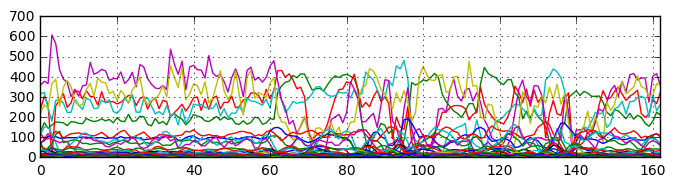
\includegraphics[width=\textwidth]{chapters/gmm/mfcc_energy_appended_cms_delta_order_2_shifted}
    \caption{MFCCs from \figureref{mfcc_energy_appended_cms_delta_order_2} shifted up. The minimum value for each feature is 1.}
    \label{fig:mfcc-shifted}
\end{figure}

\noindent After the variances are calculated, the means are shifted down,

\begin{equation}
    \mu_n = \mu_n - (1 - \min_t c_{n,t}),
    \label{eq:means-shift-down}
\end{equation}

\noindent returning to their supposed ``original" values. This procedure avoids having to shift up every vector of features, be it in the training or in the test sections, and is a practical solution to circumvent the problem.

\begin{figure}[ht]
    \centering
    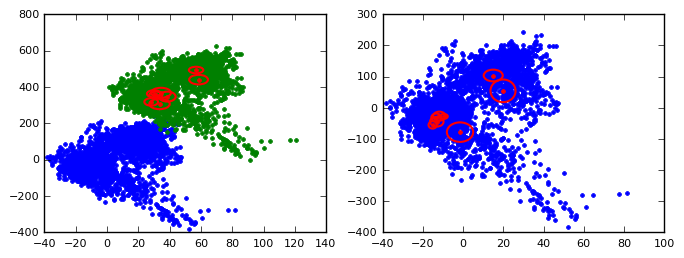
\includegraphics[width=\textwidth]{chapters/gmm/em_algorithm_r095}
    \caption{Features before (left), partitioned using k-means, and after (right) the EM algorithm. All variances (before and after EM) were calculated using FCM with $r = 0.95$. The blue points are the original features, while the greens are they shifted. Only the first deviation is shown.}
    \label{fig:frac-em_algorithm}
\end{figure}

The choice of shift up all features to 1 is mostly based in common sense. To avoid non-negative values, just shift to 0 would be sufficient. However, when $r \to 0$, the results for $X^r$ amd $\mu^r$ could fall in the indefinition $0^0$, due to approximations in floating points. Also, for values greater than or equal to 1, the exponentiation remains monotonic.